\documentclass[12pt, a4paper]{article}
\usepackage[utf8]{inputenc}
\usepackage[a4paper,lmargin=3cm,rmargin=3cm,tmargin=3cm,bmargin=3cm]{geometry}
\usepackage[]{graphicx}
\usepackage{hyperref}
\usepackage{caption}
\usepackage{subcaption} 
\usepackage{float}

\title{\textbf{Water Quality}}
\author{François-Xavier Arthaut, Ayoub Bhija\\ Achraf Hanini, Alexandre Em}
% \date{Juillet 2021}

\begin{document}

\maketitle

\section{Introduction}
Access to safe drinking-water is essential to health, a basic human right and a component of effective policy for health protection. This is important as a health and development issue at a national, regional and local level. In some regions, it has been shown that investments in water supply and sanitation can yield a net economic benefit, since the reductions in adverse health effects and health care costs outweigh the costs of undertaking the interventions.\\

\textbf{\textit{Problématique}}: Prédire si l'eau est potable ou non pour sa consommation.

\section{Exploration}
    Nous allons travailler sur un jeu de données contenant \textbf{3276 valeurs}, dont 1998 sont classées \textit{non potables} et 1278 classées \textit{potable}
        \begin{figure}[H]
           \centering
           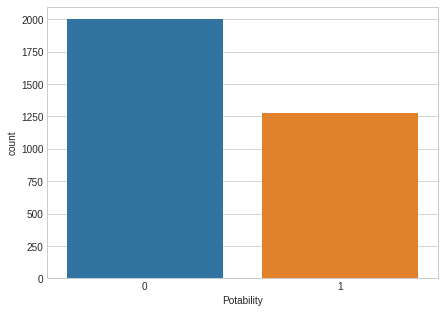
\includegraphics[width=10cm]{images/output_9_2.png}
           \caption{Nombre total d'eau potable(1) et non potable(0)}
            \label{fig:gant}
        \end{figure}
        
        
    Ce jeu de données comporte 10 colonnes:
    \begin{itemize}
        \item ph: \textit{flottant} - le pH mesure l’acidité ou la basicité d’une solution (0 to 14)
        \item Hardness: \textit{flottant} - Montant de calcium et de Magnesium dans l'eau en $mg/L$	
        \item Solids: \textit{flottant}	- le total de solide dissous dans l'eau en $ppm$
        \item Chloramines: \textit{flottant}	- montant de Chloramines en $ppm$
        \item Sulfate: \textit{flottant}	- montant de sulfate dissous en $ppm$
        \item Conductivity: \textit{flottant} - la conductivité de l'électricité de l'eau en $\mu S/cm$
        \item Organic\_carbon: \textit{flottant}	- montant de Carbone organique en $ppm$
        \item Trihalomethanes: \textit{flottant}	- montant de Trihalomethanes en $\mu g/L$
        \item Turbidity: \textit{flottant} - Mesure de l'opacité de l'eau en $NTU$ 
        \item Potability: \textit{entier} - Indique si l'eau est potable ou non
    \end{itemize} On peut voir que l'on a dans notre dataframe, que des variables quantitatives et que notre cible est un Integer dont les valeurs sont compris entre $[0,1]$  et peut être considérer comme des booleens. Nous n'aurons donc pas besoin de l'encoder.\\
    On peut aussi voir dans la figure \ref{fig:courbe_overall}, qu'il n'y a pas beaucoup de différence entre les courbes des eaux potables et non potables de chaque variable, sauf pour le \textbf{ph} et \textbf{Sulfate}. On peut donc supposer que \textbf{ph} et  \textbf{Sulfate} sont peut être des variables qui influence sur la potabilité de l'eau ou non.
    
    \begin{figure}[H]
           \centering
           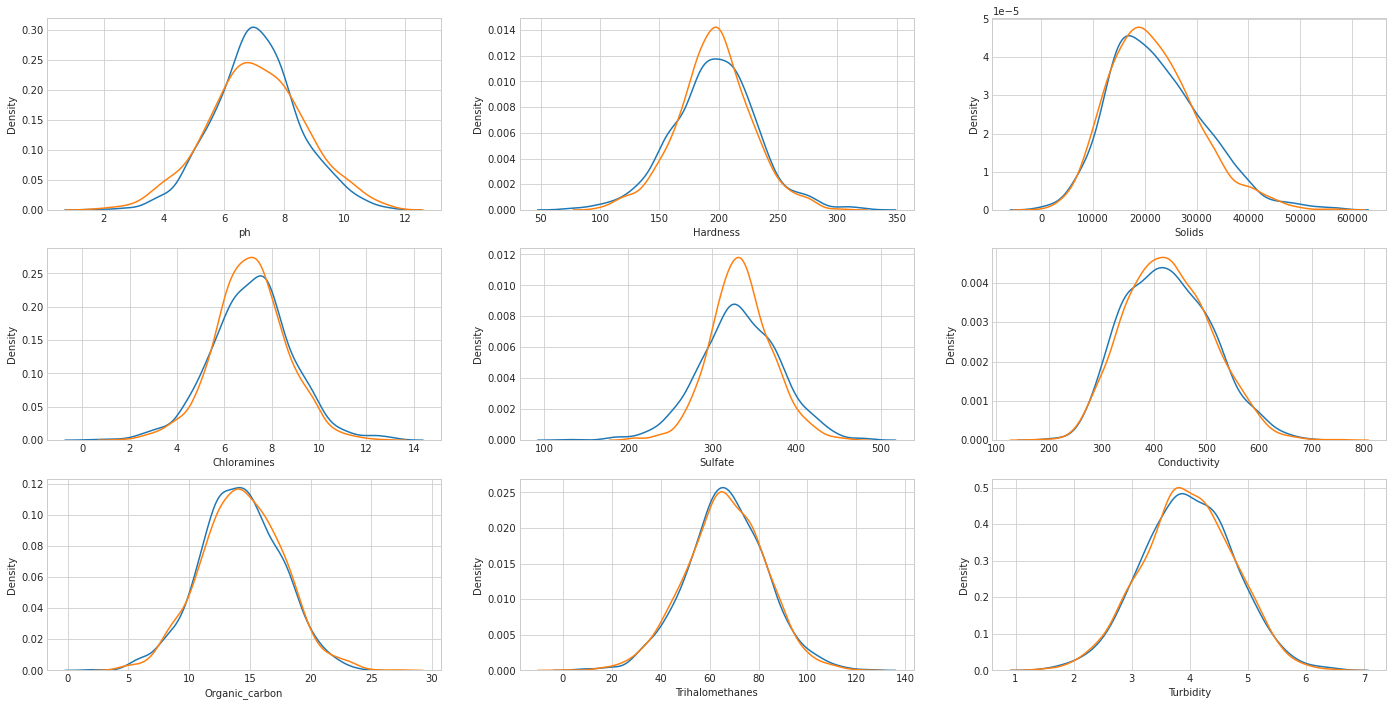
\includegraphics[width=\textwidth]{images/output_12_0.png}
           \caption{Répartition des eaux potable et non potable}
            \label{fig:courbe_overall}
    \end{figure}
    
\subsection{Quels problèmes avez-vous rencontré avec les données ?}
    \subsubsection{Valeurs nulles}
    En executant la commande \texttt{data.isnull().sum()}, nous avons pu voir que nous avions 3 variables qui contiennent des valeurs nulles (NaN):
   \begin{table}[H]
            \caption{Variables contenant des valeurs nulles (NaN)}
            \centering
            \begin{tabular}{| p{0.45\textwidth} | p{0.45\textwidth} |} 
             \hline
             \textbf{Variable} & \textbf{Occurrence de valeurs nulles} \\
             \hline
             ph & 491 \\ [.4ex] 
             \hline
             Sulfate & 781 \\ [.4ex] 
             \hline
             Trihalomethanes & 162 \\ [1ex] 
             \hline
        \end{tabular}
        \label{table:connotation weproov}
    \end{table}
    
    
    Pour un total de 1434 lignes, soit environ $44\%$ des données. Ce qui est assez conséquent si on supprime toutes ces lignes. Nous avons donc fait plusieurs cas d'essais incluant la suppression des lignes contenant les valeurs nulles. Nous avons donc remplis ces valeurs nulles par interpolation (cas 1) et par la moyenne de chaque variable (cas 2). Nous pourrons donc comparer ces 3 cas pour ne prendre uniquement celui qui obtient le meilleur accuracy.
    
    \subsubsection{Valeurs aberrantes}
    Nous avons ensuite analyser la répartition des valeurs pour chaque variable afin d'enlever toutes les valeurs aberrantes, comme nous pouvons le voir dans la figure \ref{fig:ph_curve_abb}, on sait que le ph d'un liquide peut s'étendre de 0 à 14, mais nous recherchons le ph d'une eau potable et nous considérons que le ph de l'eau ne peut atteindre des valeurs extrémités, donc nous les avons supprimés (figure \ref{fig:ph_curve_abb_rm}).
    
    \begin{figure}[H]
     \centering
     \begin{subfigure}[b]{7cm}
           \centering
           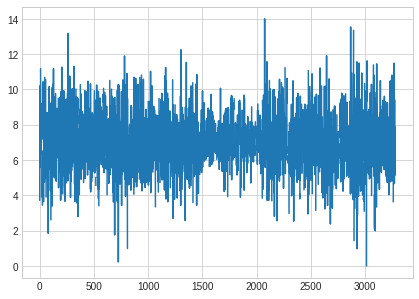
\includegraphics[width=\textwidth]{images/output_14_1.png}
           \caption{Répartition de base}
            \label{fig:ph_curve_abb}
     \end{subfigure}
     \hfill
     \begin{subfigure}[b]{7cm}
            \centering
           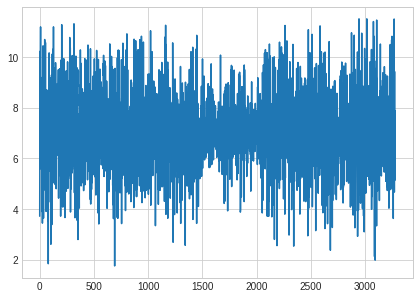
\includegraphics[width=\textwidth]{images/output_16_0.png}
           \caption{Répartition après suppression}
            \label{fig:ph_curve_abb_rm}
     \end{subfigure}
    \caption{Répartition des valeurs du ph}
    \label{fig:three graphs}
\end{figure}
    
    \subsubsection{Incohérence avec les recommandations}
    Nous avons analyser et comparer pour chaque variable, toutes les valeurs avec les recommandations données dans l'énonce et il y a beaucoup d'incohérence entre eux. Par exemple le Sulfate a une accuracy de $\sim 40\%$, mais il n'y a aucune eau non potable qui rempli les recommandations qui sont d'être compris dans $[3, 1000]$ mg/L.\\
    
    La recommandation la plus proche de la réalité est la Conductivité de l'eau avec une accuracy de $\sim 50\%$ comme on peut le voir dans la figure \ref{fig:conductivite_hist}
    
    \begin{figure}[H]
           \centering
           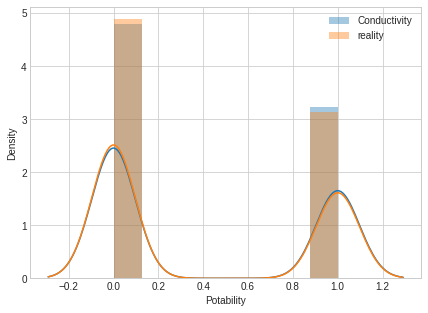
\includegraphics[width=9.5cm]{images/output_42_1.png}
           \caption{Répartition des eaux potable et non potable}
            \label{fig:conductivite_hist}
    \end{figure}
    
    Nous avons ensuite comparé chaque variable avec la cible pour voir si il y avait une corrélation entre elles (figure \ref{fig:mat_corr}) et nous avons remarqué que la correlation entre chaque variable et la cible est très faible, c'est à dire que chaque valeur s'approche de 0 et qu'aucune valeur à l'absolue n'est supérieure à 0.5 et on peut donc emettre l'hypothèse qu'ils sont independent et qu'il y a aucune relation lineaire entre elles.
    
    \begin{figure}[H]
           \centering
           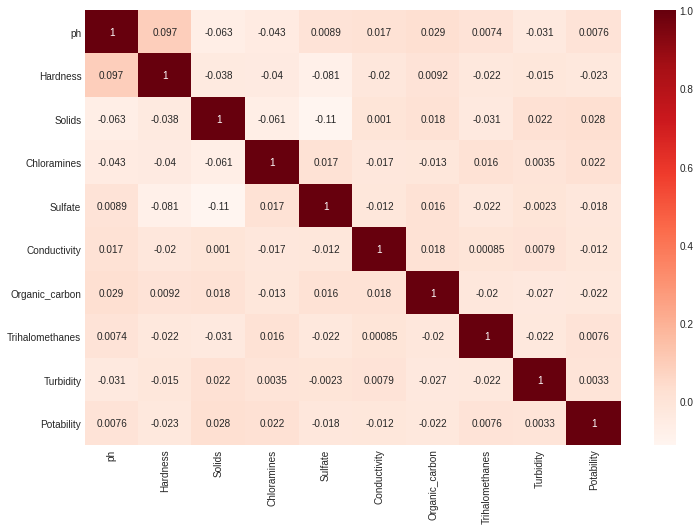
\includegraphics[width=\textwidth]{images/output_64_0.png}
           \caption{Matrice de corrélation entre variable}
            \label{fig:mat_corr}
    \end{figure}
    
    Afin de comparer au résultat final, nous avons donc fait plusieurs essai sur tout les cas de traitement (suppression des valeurs nulles, interpolation, moyennes) et sur différents modèles.
    \section{Quel(s) modèle(s) avez-vous choisi ?}
    Le but de notre projet est de prédire si une eau est potable ou non et nous voulons donc une classification de l'eau.\\
    Après avoir réaliser un traitement de nos données, nous avons étudié la matrice de corrélation pour ne sélectionner que les variables dont la corrélation est pertinente et ensuite appliquer le dataset sur un modèle de régression logistique.
    \newpage
    \subsection{Regression logistique}
    \begin{figure}[H]
           \centering
           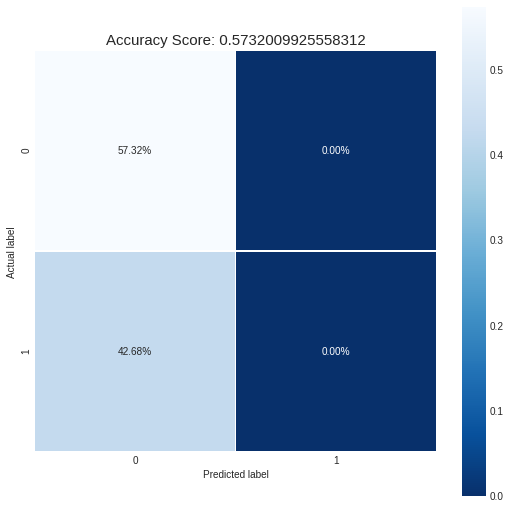
\includegraphics[width=10cm]{images/confusion_matrix_log_case0.png}
           \caption{Matrice de confusion (Pearson) dans le cas suppression des NaN}
            \label{fig:reglog_0}
        \end{figure}
    On peut remarquer que ce modèle n'est pas performant, en effet on a une accuracy de $\sim57\%$ (puis $\sim62\%$ après remplissage des valeurs nulles), mais surtout en observant la matrice de confusion, aucun positif (eau potable) n'a pas été prédit correctement. On remarque la même chose après traitement des données nulles (figure \ref{fig:mat_conf_reglog})
    \begin{figure}[H]
     \centering
     \begin{subfigure}[b]{6.75cm}
           \centering
           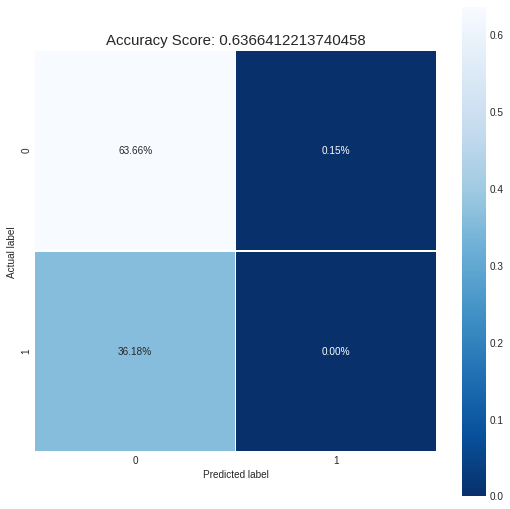
\includegraphics[width=\textwidth]{images/confusion_matrix_log_case1.png}
           \caption{Cas de remplissage par interpolation des données nulles}
            \label{fig:corr_matrix_inter}
     \end{subfigure}
     \hfill
     \begin{subfigure}[b]{6.75cm}
            \centering
           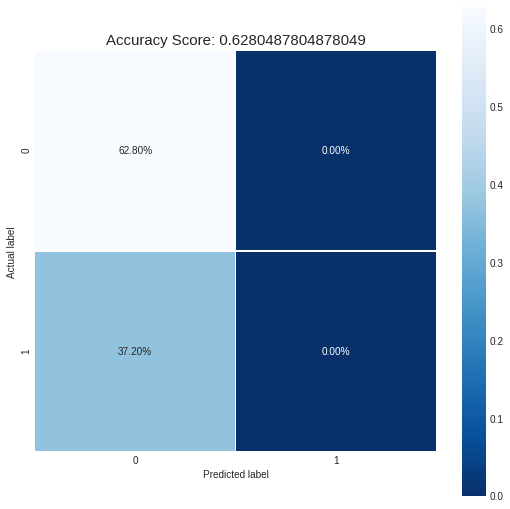
\includegraphics[width=\textwidth]{images/confusion_matrix_log_case2.png}
           \caption{Cas de remplissage par moyenne des données nulles}
            \label{fig:corr_matrix_mean}
     \end{subfigure}
    \caption{Matrices de confusion (Pearson)}
    \label{fig:mat_conf_reglog}
    \end{figure}
    
    \subsection{Decision tree}
    Afin d'avoir une meilleure visualisation, nous allons utiliser un arbre de decision et calibrer les hyperparamètres afin d'avoir un accuracy optimal sans tombé dans le cas de sur-entrainement ni de sous-entrainement, pour cela nous allons tout d'abord limiter la hauteur et le nombre de feuille de notre arbre de decision.
    \begin{figure}[H]
           \centering
           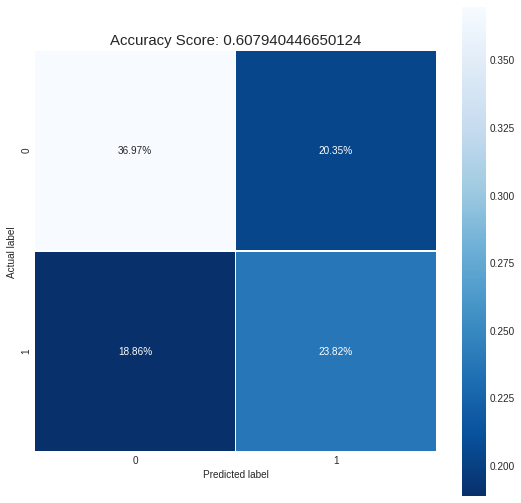
\includegraphics[width=8.5cm]{images/confusion_matrix_decTree_case0.png}
           \caption{Nombre total d'eau potable(1) et non potable(0)}
            \label{fig:dectree_0}
        \end{figure}
    
    On peut remarquer une amélioration par rapport au modèle de régression logistique. Notamment après traitement des données on peut remarquer une nette amélioration allant jusqu'à $\sim 75\%$ d'accuracy avec $\sim 19\%$ de vrai positif (f. \ref{fig:mat_conf_decTree}).
    
    \begin{figure}[H]
     \centering
     \begin{subfigure}[b]{6.75cm}
           \centering
           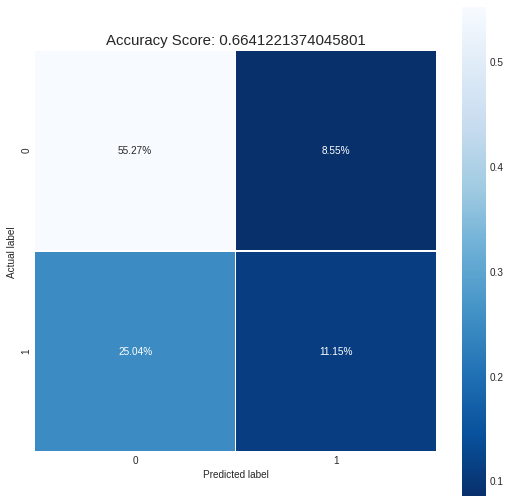
\includegraphics[width=\textwidth]{images/confusion_matrix_decTree_case1.png}
           \caption{Cas de remplissage par interpolation des données nulles}
            \label{fig:decTree_corr_matrix_inter}
     \end{subfigure}
     \hfill
     \begin{subfigure}[b]{6.75cm}
            \centering
           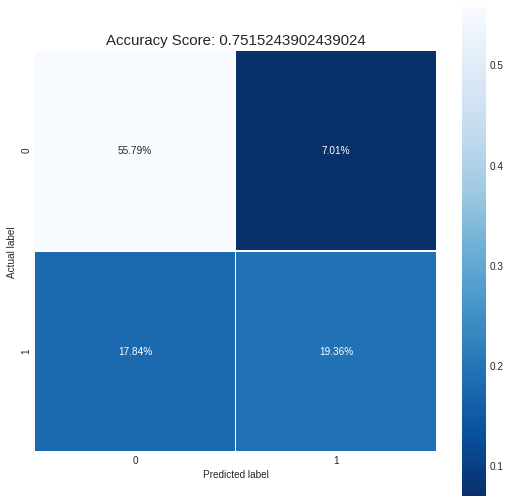
\includegraphics[width=\textwidth]{images/confusion_matrix_decTree_case2.png}
           \caption{Cas de remplissage par moyenne des données nulles}
            \label{fig:decTree_corr_matrix_mean}
     \end{subfigure}
    \caption{Matrices de confusion (Pearson)}
    \label{fig:mat_conf_decTree}
    \end{figure}
    
    Nous allons ensuite essayer d'améliorer l'accuracy compte tenu de la problématique, en essayant avec un autre modèle la forêt aléatoire.  
    
    \subsection{Random tree}
    Ayant des variables indépendantes et que ses valeurs sont éparpillés, nous allons ensuite utiliser le modèle Random forest. 
    \begin{figure}[H]
           \centering
           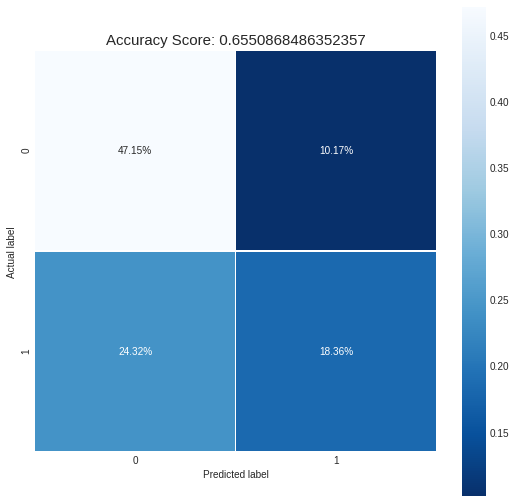
\includegraphics[width=8cm]{images/confusion_matrix_randTree_case0.png}
           \caption{Nombre total d'eau potable(1) et non potable(0)}
            \label{fig:randtree_0}
    \end{figure}
    
    Encore une fois on peut remarquer une nette amélioration par rapport aux deux autres modèle. Notamment après traitement des données on peut remarquer une nette amélioration allant jusqu'à $\sim 80\%$ d'accuracy avec $\sim 26\%$ de vrai positif.
    
    \begin{figure}[H]
     \centering
     \begin{subfigure}[b]{6.75cm}
           \centering
           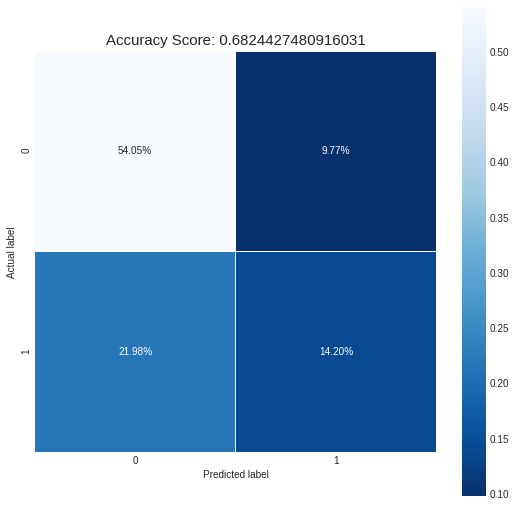
\includegraphics[width=\textwidth]{images/confusion_matrix_randTree_case1.png}
           \caption{Cas de remplissage par interpolation des données nulles}
            \label{fig:randTree_corr_matrix_inter}
     \end{subfigure}
     \hfill
     \begin{subfigure}[b]{6.75cm}
            \centering
           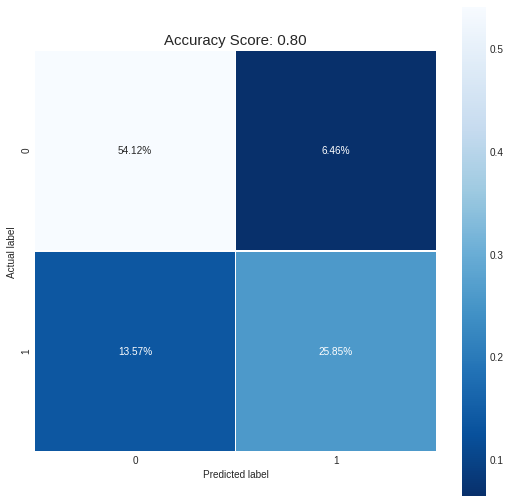
\includegraphics[width=\textwidth]{images/output_85_0.png}
           \caption{Cas de remplissage par moyenne des données nulles}
            \label{fig:randree_corr_matrix_mean}
     \end{subfigure}
    \caption{Matrices de confusion (Pearson)}
    \label{fig:mat_conf_randTree}
    \end{figure}
    A partir de ce modèle nous avons aussi tracé un histogramme des variables importantes (figure \ref{fig:imp_car}) et on comme prévu, d'après notre hypothèse énoncé au début de ce rapport. On peut voir que le Sulfate et le ph sont des variables qui sont bien importantes.
    
    \begin{figure}[H]
           \centering
           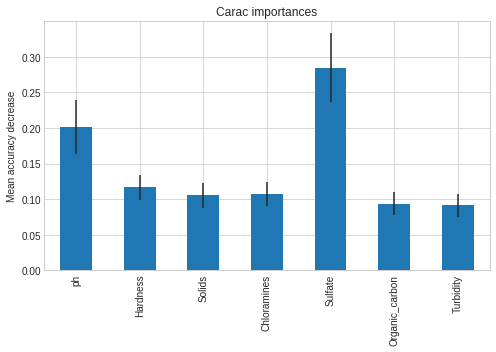
\includegraphics[width=13cm]{images/output_83_0.png}
           \caption{Histogramme des variables selon leur importance}
            \label{fig:imp_car}
    \end{figure}

    Nous avons aussi comparé ces 3 modèles par une courbe de caractéristique de performance et de taux d'erreurs des faux positifs avec les faux négatifs. 
    
    \begin{figure}[H]
           \centering
           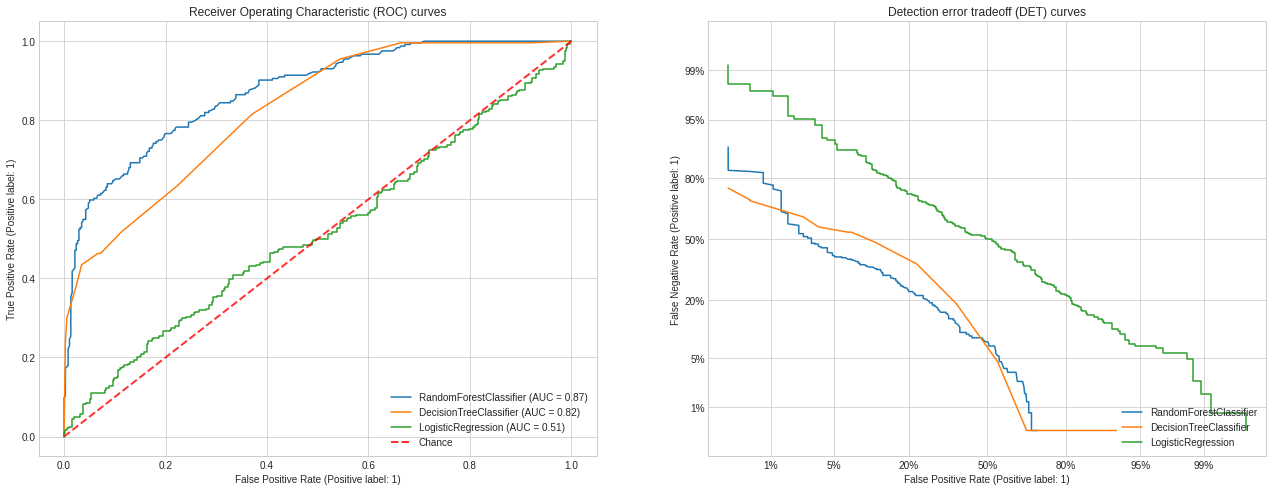
\includegraphics[width=\textwidth]{images/output_86_0.png}
           \caption{Histogramme des variables selon leur importance}
            \label{fig:ROC_DET}
    \end{figure}
    
    On peut voir dans les graphes ci dessus que l'algorithme de Random Forest est bien le plus précis par l'allure des courbes et que la courbe de DecisionTreeClassifier et de RandomForestClassifier se rapprochent et ont presque la même allure dans les deux courbes


\section{Conclusion}
En comparant différent modèle et en traitant les données de façon différente, on est passé d’une accuracy de $\sim60\%$ à une accuracy de $\sim80\%$ avec un taux de vrai positif de $\sim26\%$ grâce au model \textit{RandomForestClassifier}. Ce qui n’est pas mal étant donné le jeu de donnée que l’on a mais insuffisant étant donné la problématique qui est un enjeu majeur pour l’homme.
En effet, si une personne boit de l'eau considéré comme potable mais qui ne l'est en réalité pas, il pourrait développer des maladies plus ou moins grave. Pour toute les eaux considérées non potables alors qu'elles le sont, on priverait un village, une ville voir un pays de boire de l'eau potable.\\
On pourrait peut être améliorer l’accuracy en traitant les valeurs nulles et les valeurs aberrantes (qui ont été supprimé au cours de ce projet) plus efficacement, par exemple en comparant la ligne contenant la valeur nulle avec les autres lignes et l’affecter à la valeur de la ligne qui possède le maximum de similitude selon un degrès choisi.


\begin{thebibliography}{}
    \bibitem{dataframes} \href{https://www.kaggle.com/adityakadiwal/water-potability}{Water quality dataset}
    \bibitem{mean-nan-values} \href{https://moncoachdata.com/blog/manipulation-de-donnees-avec-pandas/}{Manipulation de données avec Pandas} - MonCoachData
    \bibitem{confusion matrix} \href{https://indiaai.gov.in/article/confusion-matrix-explained}{Confusion matrix explained - Dhilip Subramanian}
    \bibitem{decisionTree} \href{https://towardsdatascience.com/how-to-tune-a-decision-tree-f0321801680}{How to tune a decision tree} - Mukesh Mithrakumar
\end{thebibliography}
\end{document}
